\documentclass[a4paper,12pt]{article}

\usepackage{fontspec}
\usepackage{url}
\usepackage{float}
\setmainfont{Times New Roman}
\usepackage[russian]{babel}
\usepackage{graphicx}
\usepackage{geometry}
\geometry{left=3cm,right=1.5cm,top=2cm,bottom=2cm}
\usepackage{setspace}
\onehalfspacing
\setlength{\parindent}{1.25cm}

\begin{document}

\begin{titlepage}
  \thispagestyle{empty}
  \begin{center}

    
\includegraphics[width=0.18\textwidth]{../assets/gerb.png}

    \vspace{0.5cm}

    {\small
      МИНИСТЕРСТВО НАУКИ И ВЫСШЕГО ОБРАЗОВАНИЯ\\
      РОССИЙСКОЙ ФЕДЕРАЦИИ
    }

    \vspace{0.3cm}

    {\small
      Федеральное государственное бюджетное образовательное учреждение\\
      высшего образования
    }

    \vspace{0.3cm}

    {\large \textbf{«МИРЭА --- Российский технологический университет»}}

    {\normalsize РТУ МИРЭА}

    {\normalsize Институт искусственного интеллекта (ИИИ)}\\
    {\normalsize Кафедра промышленной информатики (ПИ)}

    \vspace{2cm}

    {\LARGE \textbf{ОТЧЁТ}}

    \vspace{0.3cm}

    {\Large \textbf{ПО ПРАКТИЧЕСКОЙ РАБОТЕ № 14}}

    \vspace{0.4cm}

    {\large по дисциплине «Информатика»}

    \vspace{2.5cm}

    \begin{tabular}{ll}
      Выполнил студент группы КВБО-11-25 & Шапаренко Ф.А. \\
      Принял ассистент: & Беднов Г.А. \\
    \end{tabular}

    \vfill

    Практическую работу выполнил: «05» апреля 2026 г.\\
    «Зачтено» \rule{1cm}{0.4pt} 2026 г.

    \vspace{1cm}

    Москва 2026

  \end{center}
\end{titlepage}

\noindent\textbf{Тема:} УНИВЕРСАЛЬНЫЕ ЛОГИЧЕСКИЕ МОДУЛИ\\
\noindent\textbf{Цель работы:} \\ 1. Ознакомится с концепцией LUT как
универсального логического модуля.  \\ 2. Применить LUT для реализации
булевых функций и комбинационных  устройств.  \\ 3. Реализовать
универсальный преобразователь кодов на основе шифратора и  дешифратора.

\paragraph{Вариант 27.}
$f = (a \land b \land c) \lor (\lnot a \land \lnot b)
\lor (\lnot a
\land \lnot c) \lor (\lnot b \land \lnot c)$

\begin{table}[H]
  \centering
  \caption{Таблица истинности функции, вариант 27}
  \begin{tabular}{|c|c|c|c|}
    \hline
    $a$ & $b$ & $c$ & $f$ \\
    \hline
    0 & 0 & 0 & 1 \\
    0 & 0 & 1 & 1 \\
    0 & 1 & 0 & 1 \\
    0 & 1 & 1 & 0 \\
    1 & 0 & 0 & 1 \\
    1 & 0 & 1 & 0 \\
    1 & 1 & 0 & 0 \\
    1 & 1 & 1 & 1 \\
    \hline
  \end{tabular}
\end{table}

\begin{figure}[H]
  \centering
  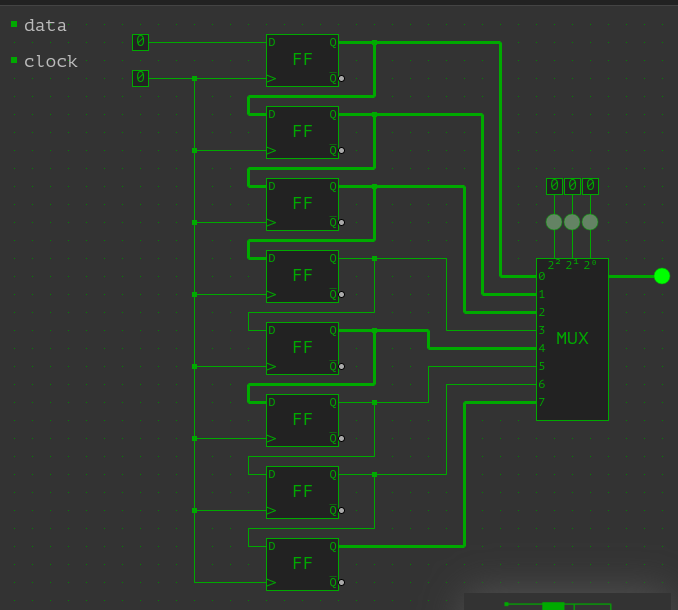
\includegraphics[width=0.8\textwidth]{../assets/14.png}
  \caption{Программируемая логика трех переменных}
\end{figure}

\begin{table}[H]
  \centering
  \caption{Таблица преобразования кодов, вариант 27}
  \begin{tabular}{|c|c|c|c|c|c|}
    \hline
    $A_2$ & $A_1$ & $A_0$ & $B_2$ & $B_1$ & $B_0$ \\
    \hline
    0 & 0 & 0 & 0 & 0 & 0 \\
    0 & 0 & 1 & 1 & 1 & 0 \\
    0 & 1 & 0 & 1 & 0 & 1 \\
    0 & 1 & 1 & 0 & 1 & 1 \\
    1 & 0 & 0 & 1 & 0 & 0 \\
    1 & 0 & 1 & 1 & 1 & 1 \\
    1 & 1 & 0 & 0 & 1 & 0 \\
    1 & 1 & 1 & 0 & 0 & 1 \\
    \hline
  \end{tabular}
\end{table}

\url{http://simulator.io/board/awVLbIHT4y/4}

\end{document}
